\documentclass[]{book}

%These tell TeX which packages to use.
\usepackage{array,epsfig}
\usepackage{amsmath}
\usepackage{amsfonts}
\usepackage{amssymb}
\usepackage{amsxtra}
\usepackage{amsthm}
\usepackage{mathrsfs}
\usepackage{color}

%Here I define some theorem styles and shortcut commands for symbols I use often
\theoremstyle{definition}
\newtheorem{defn}{Definition}
\newtheorem{thm}{Theorem}
\newtheorem{cor}{Corollary}
\newtheorem*{rmk}{Remark}
\newtheorem{lem}{Lemma}
\newtheorem*{joke}{Joke}
\newtheorem{ex}{Example}
\newtheorem*{soln}{Solution}
\newtheorem{prop}{Proposition}

\newcommand{\lra}{\longrightarrow}
\newcommand{\ra}{\rightarrow}
\newcommand{\surj}{\twoheadrightarrow}
\newcommand{\graph}{\mathrm{graph}}
\newcommand{\bb}[1]{\mathbb{#1}}
\newcommand{\Z}{\bb{Z}}
\newcommand{\Q}{\bb{Q}}
\newcommand{\R}{\bb{R}}
\newcommand{\C}{\bb{C}}
\newcommand{\N}{\bb{N}}
\newcommand{\M}{\mathbf{M}}
\newcommand{\m}{\mathbf{m}}
\newcommand{\MM}{\mathscr{M}}
\newcommand{\HH}{\mathscr{H}}
\newcommand{\Om}{\Omega}
\newcommand{\Ho}{\in\HH(\Om)}
\newcommand{\bd}{\partial}
\newcommand{\del}{\partial}
\newcommand{\bardel}{\overline\partial}
\newcommand{\textdf}[1]{\textbf{\textsf{#1}}\index{#1}}
\newcommand{\img}{\mathrm{img}}
\newcommand{\ip}[2]{\left\langle{#1},{#2}\right\rangle}
\newcommand{\inter}[1]{\mathrm{int}{#1}}
\newcommand{\exter}[1]{\mathrm{ext}{#1}}
\newcommand{\cl}[1]{\mathrm{cl}{#1}}
\newcommand{\ds}{\displaystyle}
\newcommand{\vol}{\mathrm{vol}}
\newcommand{\cnt}{\mathrm{ct}}
\newcommand{\osc}{\mathrm{osc}}
\newcommand{\LL}{\mathbf{L}}
\newcommand{\UU}{\mathbf{U}}
\newcommand{\support}{\mathrm{support}}
\newcommand{\AND}{\;\wedge\;}
\newcommand{\OR}{\;\vee\;}
\newcommand{\Oset}{\varnothing}
\newcommand{\st}{\ni}
\newcommand{\wh}{\widehat}

%Pagination stuff.
\setlength{\topmargin}{-.3 in}
\setlength{\oddsidemargin}{0in}
\setlength{\evensidemargin}{0in}
\setlength{\textheight}{9.in}
\setlength{\textwidth}{6.5in}
\pagestyle{empty}



\begin{document}


\subsection*{Exo 1}
\subsubsection*{Q preliminaire}
Un mouvement rectiligne et uniforme.

\subsubsection*{Q 1.1 part 1}
(a) $v(t) = v_0 + a_0.t$ avec $v_0$ la vitesse initiale de la pierre et $a_0$ l'acc\'ec\'el\'eration


(b) $x(t) = v_0.t + 1/2.a_0.t^2$. Comme la pierre est lance de l'origine $x_0 = 0$.


(c) La pierre doit s'arr\^eter sur la cible donc $v(t)=0m/s$ (la pierre est stationaire) 
et $x(t) = l = 28m$ la distance du centre de la cible. Donc, il faut r\'esoudre:
$$
\left\{ 
\begin{array}{l}
0 = v_0 + a_0.t \\
l = v_0.t + 1/2.a_0.t^2\\
\end{array}
\right. 
$$

$$
\left\{ 
\begin{array}{l}
v_0 = - a_0.t \\
l = v_0.t + 1/2.a_0.t^2\\
\end{array}
\right. 
$$

$$
\left\{ 
\begin{array}{l}
v_0 = - a_0.t \\
l = - a_0.t^2 + 1/2.a_0.t^2\\
\end{array}
\right. 
$$

$$
\left\{ 
\begin{array}{l}
v_0 = - a_0.t \\
t = \sqrt{\frac{l}{-1/2.a_0}} = \sqrt{\frac{-2.l}{a_0}}\\
\end{array}
\right. 
$$

$$
\left\{ 
\begin{array}{l}
v_0 = - \sqrt{-2.l.a_0} \\
t = \sqrt{\frac{l}{-1/2.a_0}} = \sqrt{\frac{-2.l}{a_0}}\\
\end{array}
\right. 
$$

Donc $v_0 = 2.245m/s$ et $t=24.94s$. 

\subsubsection*{Q 1.1 part 2}
(a) $a = \lambda . v$, donc $m/s^2 = \lambda . m/s$. Donc, l'unit\'e de $\lambda$ est $s^{-1}$.


(b)On a $\frac{dv}{dt} = a$, donc $\frac{dv}{dt} = -\lambda\, v$ ou $\frac{dv}{dt} + \lambda\, v = 0$. 
La solution d'une \'equation diff\'erentielles du premier ordre est $Ce^{kt}$. 
Prenons $v(t) = Ce^{kt}$. A $t=0$, la vitesse initiale
est $v_0$. Ce qui fait $v_0 = Ce^{k.0}$, donc $C = v_0$. 


En remplacant $v$ par sa valeur dans l`\'equation diff\'erentielles, on a 
$$ \frac{d\, v_0e^{kt}}{dt} + \lambda\, v_0e^{kt} = 0$$
$$ k.v_0e^{kt} + \lambda\, v_0e^{kt} = 0$$
$$ v_0e^{kt}(k + \lambda) = 0$$
$$ k = -\lambda $$

Par cons\'equent $v(t) = v_0.e^{-\lambda\, t}$

(c) on a $\frac{dx}{dt} = v$. Donc $\frac{dx}{dt} = v_0.e^{-\lambda\, t}$. 
$$x(t) =  \frac{-v_0}{\lambda}e^{-\lambda\, t}$$

\subsubsection*{Q 1.2 part 1}
(a) Oui, la vitesse initiale sur la figure 2 (2.25 m/s) est du m\^eme ordre de grandeur que la 
valeur calcul\'ee (2.45 m/s). La vitesse d\'ecroit selon une presque une droite ce qui indique 
que l'acc\'el\'eration est constante. La pente de la droite est environ de ($(0-2.25)/(22-0) = -0.1\,m/s^2$
qui est proche de $0.09\,m/s^2$


(b) \`A l'instant $t=7s$. la vitesse devient constante ce qui indique un changement dans l'acceleration
pendant 2 secondes puis l'acc\'el\'eration redevient identique. AU m\^eme instant, 
la pierre change de trajectoire et acc\'el\`ere sur l'axe $O_y$.


(c) Entre les instants 0 et 15s la vitesse d\'ecroit lin\'eairement. L'\'equation de la vitesse 
est $v(t) = v_0 - at = 2.25 - 0.1t$. L'\'equation horaire $x(t)$ est $2.25t - 0.05t^2 + x_0$. 
\`A l'instant $t = 0$, la pierre se trouve sur l'origine de l'axe donc:
$$ x(t) = 2.25t - 0.05t^2$$
 
\subsubsection*{Q 1.2 part 2}
(a) Entre les instants 0 et $t_1$, la vitesse oscille autour de $0m/s$,


(b) Pour $t \in [0,t_1], y(t) = 0.t+C_1=C_1$. \`A l]instant $t=0$, la pierre se trouve \`a l'origine, $y(0)= 0 = C_1$. Donc entre $[0,t_1], \; y(t) = 0$. 

(c) $v_y$ repr\'esente une vitesse, son unit\'e est $m/s$. $\tau$ est le param\`etre de 
l'\'equation $v_y(t)$. Son unit\'e est en seconde. L'\'equation est $m/s = k_0 + k1*s + k_2*s^2$, 
donc $k_0$ est en $m/s$, $k_1$ est en $m/s^2$ et $k_2$ est en $m/s^3$.

(d)
$$ v(t) =
\left\{ 
\begin{array}{l l}
0 &  t \in [0,t_1] \\
k_0 + k1*\tau + k_2*\tau^2  &  t \in ]t_1,t_2], \tau = t - t_1 \\
\end{array}
\right. 
$$

$$ v(t) =
\left\{ 
\begin{array}{l l}
0 &  t \in [0,8] \\
1.1 - 0.22*\tau + 0.01*\tau^2  &  t \in ]8,11], \tau = t-8 \\
\end{array}
\right. 
$$

(e) L'\'equation est
$$ v(t) =
\left\{ 
\begin{array}{l l}
0 &  t \in [0,8] \\
1.1 - 0.22*\tau + 0.01*\tau^2  &  t \in ]8,11], \tau = t-8 \\
-0.1  &  t \in ]11,15] \\
\end{array}
\right. 
$$

\subsubsection*{Q 1.2 part 3}
\begin{itemize}
\item Vitesse nulle entre 0 et 8, donc pas de d\'eplacement sur $O_y$.
\item Entre 8 et 11, il faut int\'egrer la vitesse, donc $y(t) = 1.1*\tau - 0.22/2*\tau^2 + 
0.01/3*\tau^3 + C_2$. A'instant $t=8$, la distance $y(8) = 0$ car pas de d\'eplacement 
sur $O_y$ entre 0 et 8 s. $y(8) = 1.1*\tau - 0.22/2*\tau^2 + 0.01/3*\tau^3 + C_2 = 0$. Donc $C_2 = 0$.
\item Entre 11 et 15, la vitesse constante donc d\'eplacement lin\'eaire. $y(t) = -0.1*\tau_2+C_3, \, \tau_2 = t-11$. \`A l'instant $t=11$, la distance $y(11) =  1.1*\tau - 0.22/2*\tau^2 + 0.01/3*\tau^3 = 1.1*3 - 0.22/2*3^2 + 0.01/3*3^3 = 2.32 =C_3$. Donc $y(t) = -0.1*\tau_2+2.32$.

\end{itemize}


$$ y(t) =
\left\{ 
\begin{array}{l l}
0 &  t \in [0,8] \\
1.1*\tau - 0.22/2*\tau^2 + 0.01/3*\tau^3 &  t \in ]8,11],\, \tau = t-8 \\
-0.1*\tau_2+2.32 &  t \in ]11,15],\, \tau_2 = t-11 \\
\end{array}
\right. 
$$

\begin{figure}[h!]
  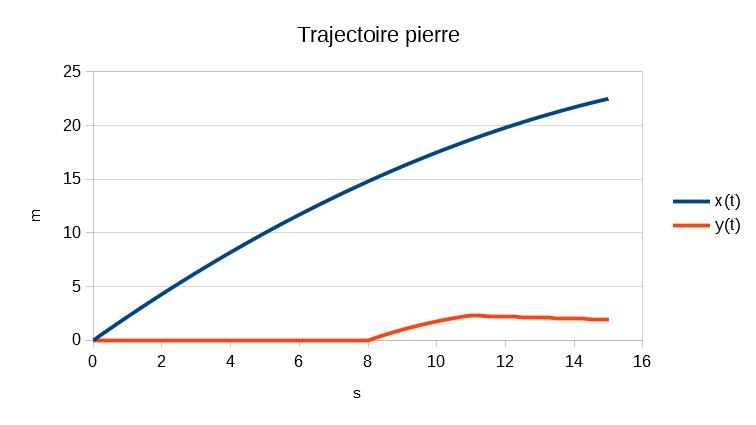
\includegraphics[width=1\linewidth]{DM1_graph1.jpg}
\end{figure}



\subsection*{Exo 2}
\subsubsection*{Q 2.1}
(1) Oui.


(2) Dans le rep\`ere $\mathcal{R}$ le marin est immobile sur l'axe $x$ et il se trouve \`a l'origine du rep\`ere.
Sur l'axe $y$, le marin descend \`a vitesse constante \`a partir de la hauteur $h$. Donc, 
$$ 
\left\{ 
\begin{array}{l}
x(t) = 0 \\
y(t) = h -0.5t \\
\end{array}
\right. 
$$

\subsubsection*{Q 2.2}
(1) Oui.

(2) Dans le rep\`ere $\mathcal{R'}$ Sur l'axe $x$, le marin se d\'eplace \`a la vitesse du bateau. Cette vitesse est 
constante donc son acc\'el\'eration est nulle.
Sur l'axe $y$, le marin descend \`a vitesse constante \`a partir de la hauteur $h$. Donc,son acc\'el\'eration est nulle.  
Par cons\'equent, les \'equations sont:
$$ a(t)
\left\{ 
\begin{array}{l}
a_x(t) = 0 \\
a_y(t) = 0 \\
\end{array}
\right. 
$$

$$ v(t)
\left\{ 
\begin{array}{l}
v_x(t) = 0*t + 3 = 3 \\
v_y(t) = 0*t - 0.5 = -0.5 \\
\end{array}
\right. 
$$


(3) Du (2), les \'equations de la trajectoire sont
$$
\left\{ 
\begin{array}{l}
x(t) = 3*t \\
y(t) = h - 0.5*t \\
\end{array}
\right. 
$$

QED.

\end{document}

